% AIPV 2026 talk scaffold (Beamer).
% Package choices mirror /Users/cheng-huiweng/Projects/aplas2024-poster/forteApr22/forteApr22.tex
% (no \input from that tree; document class here is beamer, not llncs).
\PassOptionsToPackage{fleqn}{amsmath}
\documentclass[10pt,aspectratio=169]{beamer}

\usetheme{Madrid}
\usecolortheme{default}
% Match serif math/text feel of newtx in the LLNCS source.
\usefonttheme{professionalfonts}

\usepackage[T1]{fontenc}
\usepackage{etoolbox}
\usepackage{array}
\usepackage{graphicx}
\usepackage{url}
\usepackage{tikz}
\usepackage{tikz-cd}
\usepackage{newtxtext,newtxmath}
\usepackage{xcolor}

\usepackage{hyperref}
\hypersetup{colorlinks=true,linkcolor=blue,urlcolor=blue,citecolor=blue}
\renewcommand\UrlFont{\color{blue}\rmfamily}
\urlstyle{rm}

\graphicspath{{./images/}}

\title{AIPV 2026 slides (scaffold)}
\subtitle{Inverting the formalization workflow — replace with final title}
\author{Cheng-Hui Weng}
\institute{Nagoya University}
\date{May 2026}

\begin{document}

\begin{frame}
  \titlepage
\end{frame}

\begin{frame}{Outline}
  \tableofcontents
\end{frame}

\section{MPC at a glance}

\begin{frame}{Multi-party computation (high level)}
  \begin{itemize}
    \item Parties hold \textbf{private inputs} and want a function of those inputs.
    \item Security: limit what an adversary learns from their \textbf{view} (messages, corrupt parties).
    \item \textbf{Correctness:} local pieces + reconstruction $\Rightarrow$ same result as ideal $f(\text{inputs})$.
  \end{itemize}
\end{frame}

\begin{frame}[fragile]{MPC correctness diagram}
  \centering
  \begin{tikzcd}
    E \arrow[r, "\pi_S"]
      \arrow[d, "\pi_X"']
      \arrow[dr, "\pi_{\mathrm{out}}"{pos=0.4}]
    & \prod_{i=1}^n S_i \arrow[d, "\rho"]
    \\
    \prod_{i=1}^n X_i \arrow[r, "f"'] & Y
  \end{tikzcd}
  \vspace{0.6em}

  {\small Correctness: $\rho \circ \pi_S = f \circ \pi_X = \pi_{\mathrm{out}}$.}
\end{frame}

\begin{frame}[fragile]{MPC ambient diagram (adversarial views)}
  \centering
  \begin{tikzcd}[row sep={2.8em,between origins}, column sep=large]
  & E
    \arrow[r, "\pi_S"]
    \arrow[d, "\pi_X"']
    \arrow[dl, "\pi_{X_H}"'{pos=0.45}]
    \arrow[rr, bend left=18, "\pi_{\mathrm{full}}"{pos=0.55}]
    \arrow[rrr, bend left=22, "\pi_A"{pos=0.55}]
    \arrow[dr, "\pi_{\mathrm{out}}"{pos=0.35, bend right=20}]
  & \prod_{i=1}^n S_i \arrow[d, "\rho"]
  & B_{\mathrm{full}}
    \arrow[l, "\mathrm{proj}_S"']
    \arrow[r, "\mathrm{proj}_A"]
    \arrow[dl, "\rho \circ \mathrm{proj}_S"{pos=0.6}]
  & B_A \arrow[l, "\iota_A"', hook, bend left=35]
  \\
  X_H
  & \prod_{i=1}^n X_i \arrow[l, "\mathrm{proj}_{X_H}"] \arrow[r, "f"']
  & Y
  &
  &
  \end{tikzcd}
\end{frame}

\section{How this project started}

\begin{frame}{Background (before covering spaces)}
  \begin{itemize}
    \item I had \textbf{not} formally studied topology, group theory, or covering spaces.
    \item I did know the \textbf{MPC-shaped goal}: several parties, local data, global reconstruction, control what leaks.
    \item I started with a \textbf{rough search}: what mathematical objects ``look like'' that protocol pattern?
  \end{itemize}
\end{frame}

\begin{frame}{Covering spaces and a surjective hook}
  \begin{itemize}
    \item \textbf{Covering spaces} stood out: a \textbf{covering map} is a surjection with structured fibers/sheets---reconstruction and hidden structure are already part of the picture.
    \item That surjective map was what \textbf{caught my attention} first (not a claim of prior domain mastery).
  \end{itemize}
\end{frame}

\begin{frame}{Hypothesis and workflow choice}
  \begin{itemize}
    \item \textbf{Working hypothesis:} any \textbf{surjection} (more abstractly, an \textbf{epimorphism} in a suitable category) between structured sets might admit a ``secret hiding + authorized reconstruction'' reading worth testing.
    \item Rather than spending years on pen-and-paper prerequisites first, I began to \textbf{develop and practice} \emph{formalization as a prototyping method}: state the connection in Rocq early, let the checker compress nonsense quickly, and \textbf{learn the mathematics on demand} from each iteration.
  \end{itemize}
\end{frame}

\section{Method}

\begin{frame}{LLM workflow (implementation loop)}
  \begin{enumerate}
    \item \textbf{Plan drafting:} propose a formalization plan for the target math idea.
    \item \textbf{Plan audit:} analyze why the plan should work, where it may fail, and what parts are hard; use related-work search + reasoning.
    \item \textbf{Human gate:} if the human accepts the audited plan, start formalization implementation in Rocq.
    \item \textbf{Failure recovery:} if the strategy is found logically unsound or stalls during proofs, propose a revised plan and re-audit.
  \end{enumerate}
  \vspace{0.6em}
  \begin{itemize}
    \item \textbf{Human role:} judgment \emph{and} learning from each iteration.
  \end{itemize}
\end{frame}

\begin{frame}{Roles and plan-replan feedback loop}
  \begin{center}
    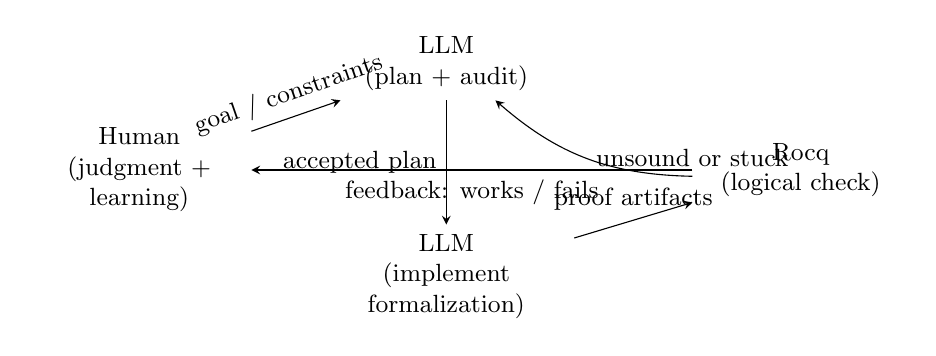
\begin{tikzpicture}[>=stealth, every node/.style={font=\small}]
      \node (H) at (0,0) {\parbox{2.6cm}{\centering Human\\(judgment + learning)}};
      \node (P) at (3.9,1.35) {\parbox{2.8cm}{\centering LLM\\(plan + audit)}};
      \node (I) at (3.9,-1.35) {\parbox{3.0cm}{\centering LLM\\(implement formalization)}};
      \node (R) at (8.4,0) {\parbox{2.5cm}{\centering Rocq\\(logical check)}};

      \draw[->] (H) -- node[above,sloped]{goal / constraints} (P);
      \draw[->] (P) -- node[left]{accepted plan} (I);
      \draw[->] (I) -- node[above]{proof artifacts} (R);
      \draw[->] (R) -- node[below,sloped]{feedback: works / fails} (H);
      \draw[->] (R) to[bend left=20] node[right]{unsound or stuck} (P);
    \end{tikzpicture}
  \end{center}
  \vspace{0.4em}
  \begin{itemize}
    \item \textbf{Replan trigger:} failed obligations can imply missing assumptions, wrong statements, or weak automation; the LLM re-audits and proposes a new plan.
  \end{itemize}
\end{frame}

\section{Glossary (non-Rocq audience)}

\begin{frame}{Terms}
  \begin{description}
    \item[Proof assistant] Environment for writing checked mathematics (here: Rocq).
    \item[Machine-checked proof] A proof the assistant has fully verified.
    \item[Axiom] Assumption accepted without proof (stated explicitly).
    \item[Placeholder proof] Informal name for skipping a proof (Rocq: \texttt{Admitted}).
  \end{description}
\end{frame}

% Add \section{} blocks and \begin{frame} ... \end{frame} as needed.

\end{document}
